\documentclass{article}

% para usar codificación utf8
% \usepackage[utf8]{inputenc}
% define los márgenes del documento
\usepackage{geometry}
  \geometry{
    a4paper,
    left = 3cm,
    right = 3cm,
    top = 2.5cm,
    bottom = 2.5cm
  }
% se usan para darle color los títulos y subtítulos
\usepackage{titlesec}
\usepackage{color}
% permite añadir imágenes al documento
\usepackage{graphicx}
% traduce textos como "figure" al español
\usepackage[spanish]{babel}

% títulos de color azul y subtítulos de color rojo
\titleformat*{\section}{\normalfont\Large\bfseries\color{blue}}
\titleformat*{\subsection}{\normalfont\large\bfseries\color{red}}
% párrafos sin sangría
\setlength\parindent{0pt}

% comandos nuevos para comillas simples y dobles
\newcommand{\simple}[1]{`#1'}
\newcommand{\doble}[1]{``#1''}

\title{Resumen Python 3}
\author{Víctor Mardones Bravo}
\date{Febrero de 2021}

\begin{document}

  % la primera hoja no tiene números de página
  \pagenumbering{gobble}

  % brujería para centrar el título y logo
  \null
  \nointerlineskip
  \vfill
  \let\snewpage \newpage
  \let\newpage \relax
  % se centra el logo svg exportado con Inkscape
  {\centering\def\svgwidth{\columnwidth}
  \input{logo python\\python-logo-inkscape.pdf_tex}}
  \maketitle
  \let \newpage \snewpage
  \vfill 
  \break

  \newpage

  % el resto del documento tiene números de página
  \pagenumbering{arabic}

  \section{Introducción a Python}

    \subsection{¿Qué es Python?}

    Python es un lenguaje de programación de alto nivel, con aplicaciones en numerosas áreas, incluyendo programación web, scripting, computación científica e inteligencia artificial.

    Es muy popular y usado por organizaciones como Google, la NASA, la CIA y Disney.

    No hay limitaciones en lo que se puede construir usando Python. Esto incluye aplicaciones autónomas, aplicaciones web, juegos, ciencia de datos, modelos de machine learning y mucho más.

    Dato curioso: Según el creador Guido van Rossum, el nombre de Python viene de la serie de comedia británica \doble{El Circo Volador de Monty Python}.

    \subsection{El Zen de Python}

      El Zen de Python es una colección de 19 \doble{principios} para escribir programas de computadores que influenciaron el diseño y representan la filosofía de este lenguaje de programación.

      \begin{figure}[ht!]
        
\includegraphics[width=\linewidth]{imagenes\\cap1\\import this.png}
        \caption{El Zen de Python se muestra en pantalla la primera vez que se ejecute esta línea.}
      \end{figure}

      \begin{figure}[ht!]
        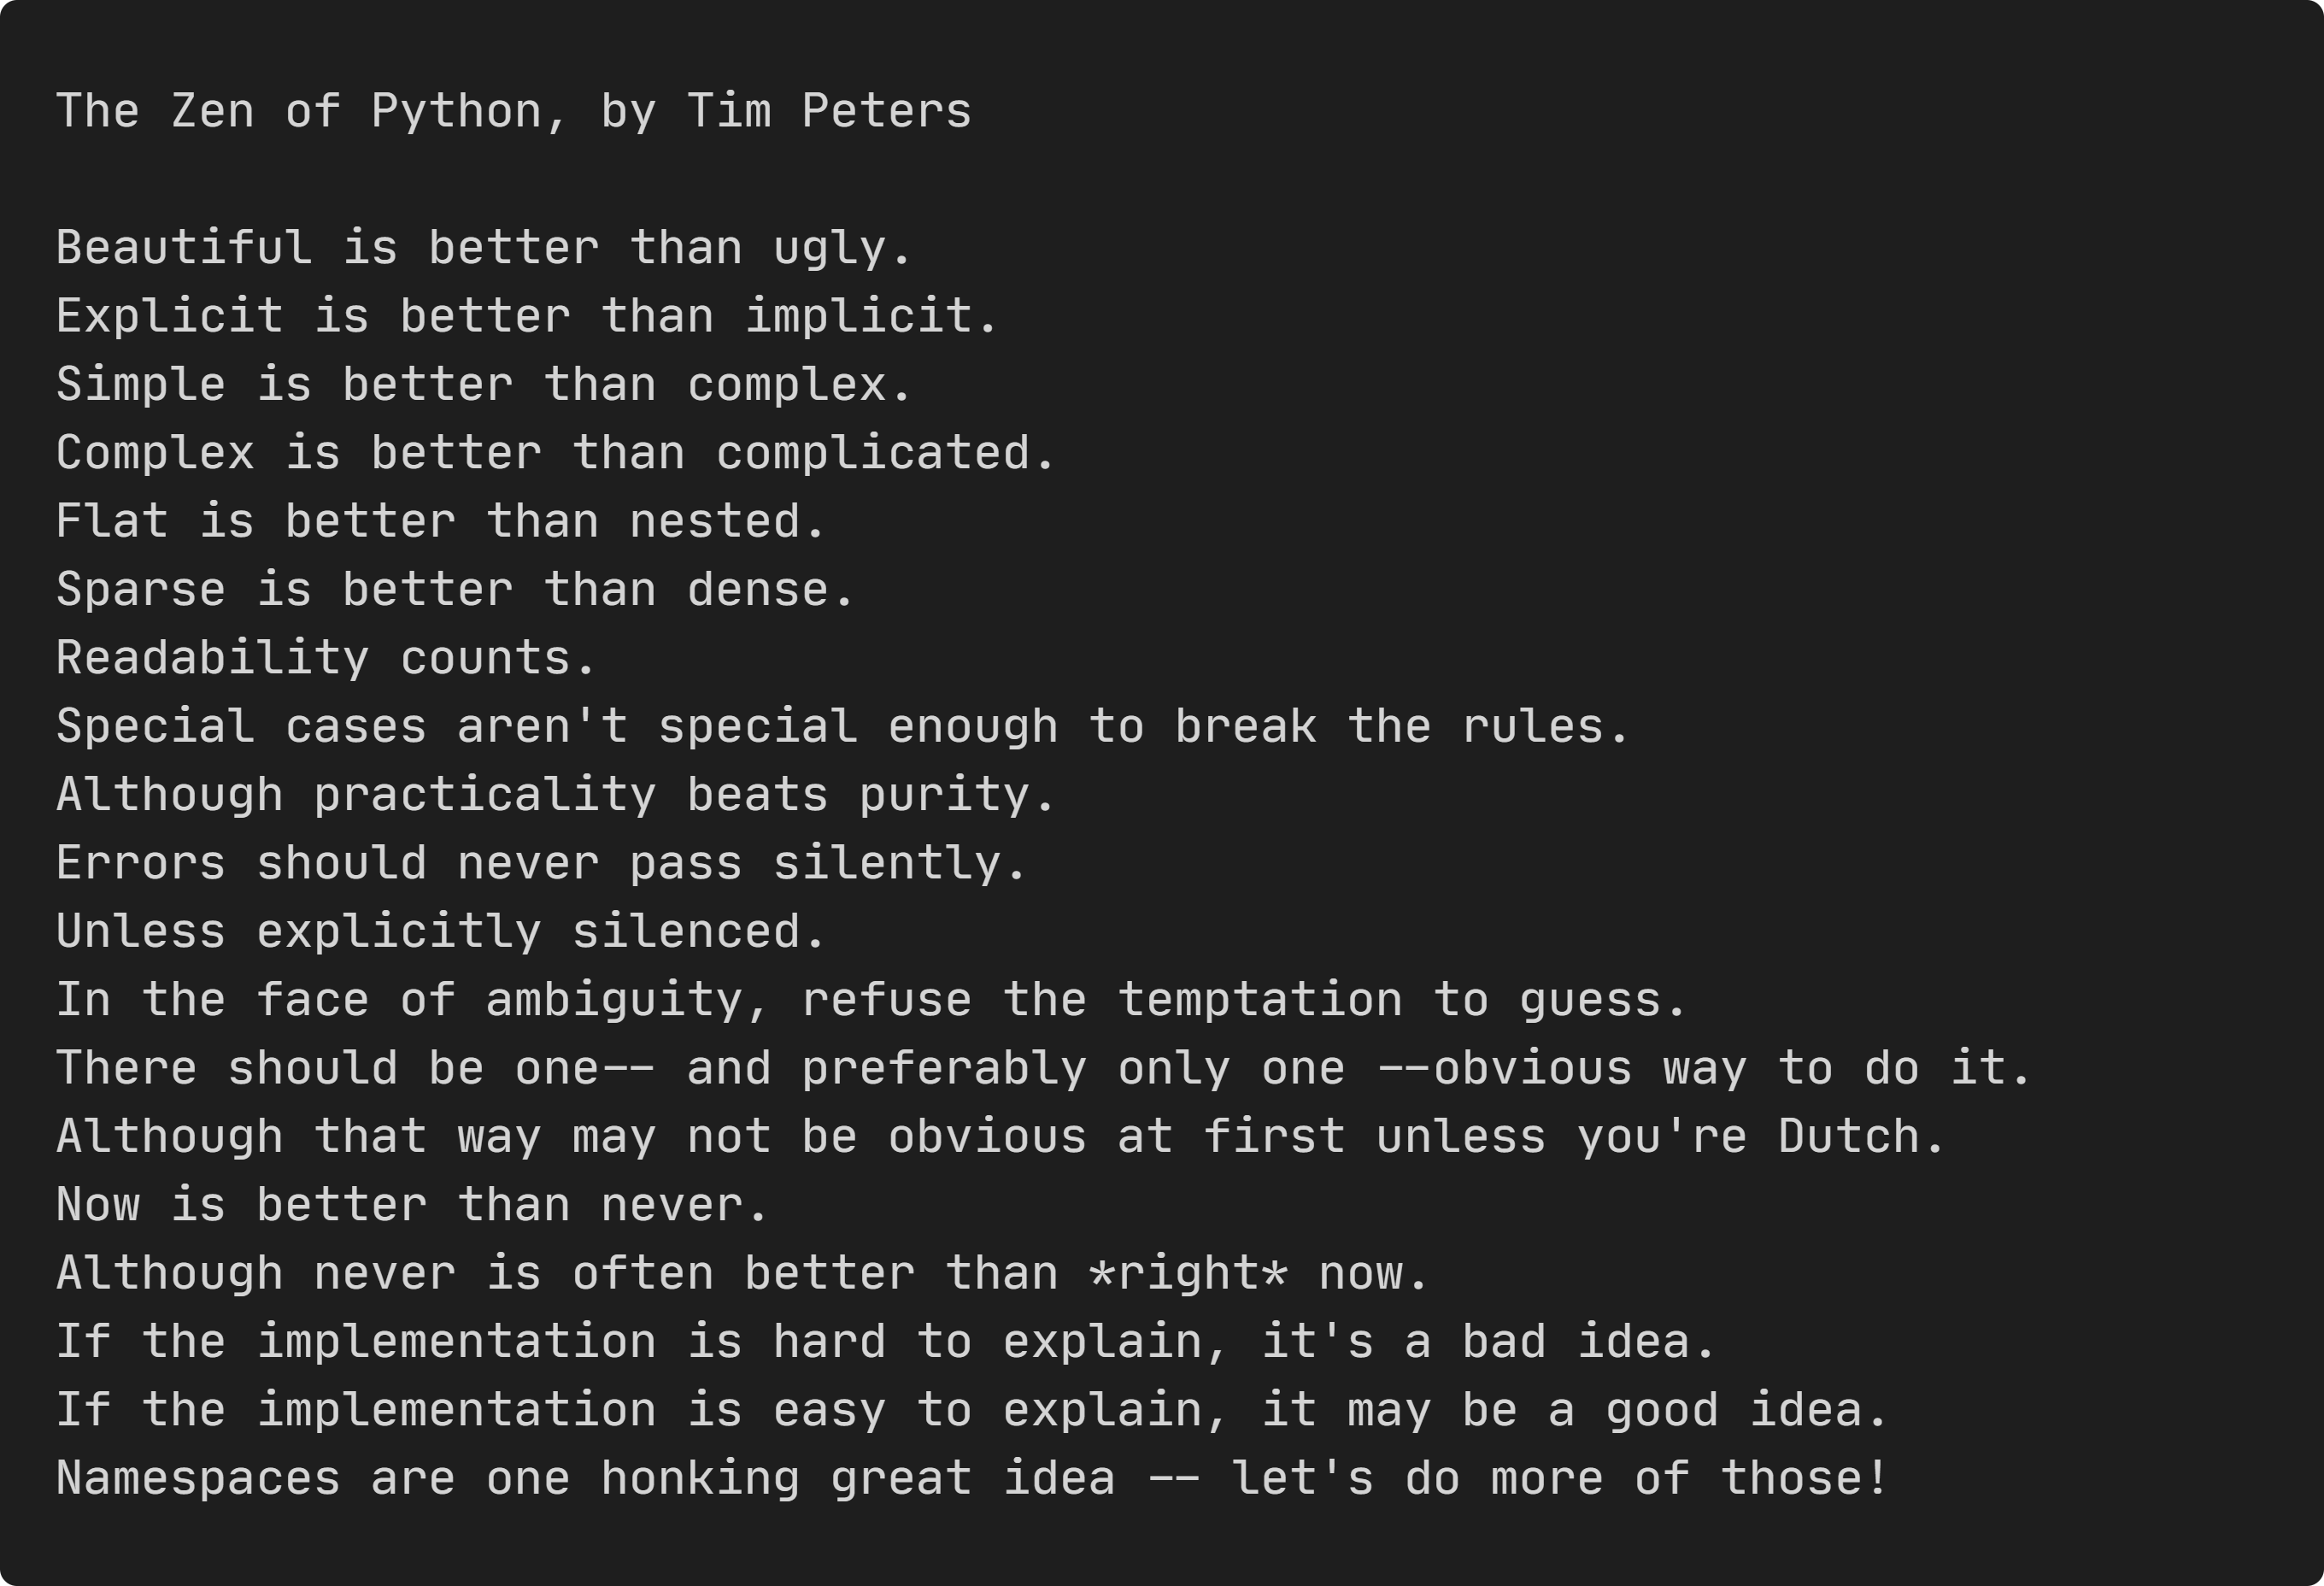
\includegraphics[width=\linewidth]{imagenes\\cap1\\zen.png}
        \caption{El Zen de Python, escrito por Tim Peters.}
      \end{figure}


    \subsection{Hola mundo}

      Para mostrar el texto \doble{Hola mundo} en pantalla se puede usar la función print().

      \begin{figure}[ht!]
        
\includegraphics[width=\linewidth]{imagenes\\cap1\\hola mundo 1.png}
        \caption{Hola mundo, el clásico primer programa en cualquier lenguaje de programación.}
      \end{figure}

      \begin{figure}[ht!]
        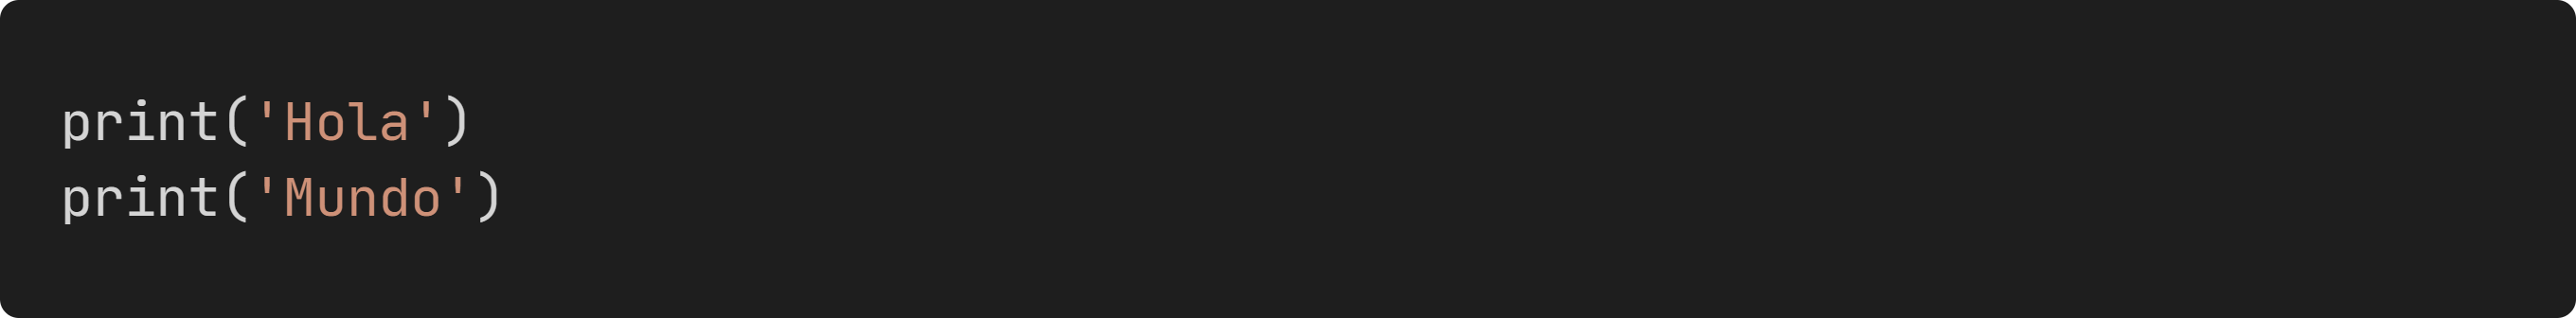
\includegraphics[width=\linewidth]{imagenes\\cap1\\hola mundo 2.png}
        \caption{Cada declaración de impresión print() genera texto en una nueva línea.}
      \end{figure}

  \newpage
  \section{Conceptos básicos}

    \subsection{Comentarios}

      Los comentarios son anotaciones en el código utilizadas para hacerlo más fácil de entender. No afectan la ejecución del código.

      En Python, los comentarios comienzan con el símbolo \#. Todo el texto luego de este \# (dentro de la misma línea) es ignorado.

      \begin{figure}[ht!]
        
\includegraphics[width=\linewidth]{imagenes\\cap2\\comentario.png}
        \caption{Ejemplo de un comentario en Python.}
      \end{figure}

      Python no soporta comentarios multilínea, al contrario de otros lenguajes de programación.

\end{document}